% !TeX spellcheck = da_DK
\subsection{Filter}
\subsubsection{Teori og design}
%Efter signalet er blevet forstærket skal det filtreres, så alle de uønskede signaler kan dæmpes. Der benyttes kun et lavpasfilter, da det ønskede signal ifølge litteraturen kan ligge i frekvensområdet $0-10$Hz, som beskrevet i afsnit \ref{FilterAfs} på side \pageref{FilterAfs}. Jævnfør pilotforsøget i afsnit \ref{Sec:PilotforsoegKort}, side \pageref{Sec:PilotforsoegKort} blev der målt et signal i frekvensområdet $0-25$Hz og det frekvensområdet sættes derfor til $0-25$Hz, for at filtrere uønskede signaler fra. 
Filtre kan udarbejdes både i aktiv og passiv form. Hvis signalet ligger i frekvensområdet under $1$MHz anbefales det at benytte aktive filtre. Aktive filtre benytter operationforstærkere, kondensatorer og modstande, hvor passive filtre benytter kondensatorer, modstande og spoler. \cite{Carter2013} Der findes flere forskellige typer filtre, heriblandt Butterworth-, Tschebyschev- og Besselfilter. Butterworthfilteret giver maksimal fladhed i pasbåndet og stopbåndet. Tschebyschevfilteret giver den hurtigste overgang fra pasbåndet til stopbåndet. Besselfilteret giver en lineær faserespons, hvilket vil sige at fasen er lineær med frekvensen.\fxnote{Til os: Fasen angiver hvor godt et signals frekvensspektrum bliver gengivet}\fxnote{skal vi have et billede ind af de forskellige typer?} \cite{Carter2013} I dette projekt anvendes et Butterworthfilter, da der ønskes maksimal fladhed i pasbåndet og stopbåndet som nævnt i kravspecifikationerne for filtret. De forskellige typer filtre fremgår af nedenstående \figref{fig:type_filtre}. \fxnote{kilde?}

\begin{figure}[H]
	\centering
	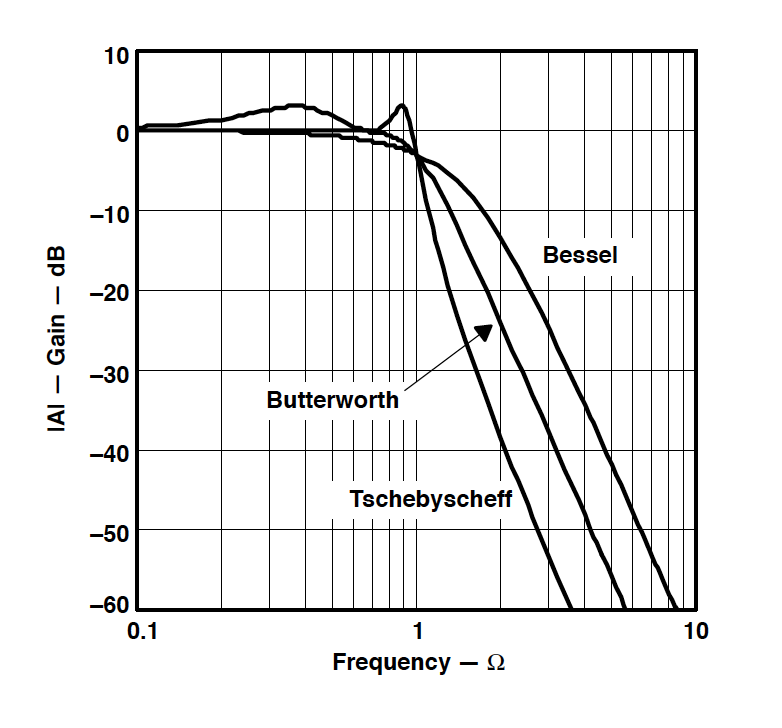
\includegraphics[scale=0.7]{figures/cProblemloesning/type_filtre.PNG}
	\caption{Figuren viser et bodeplot filter, hvor de fire karakteristika af et lavpasfilter er angivet. \cite{Carter2013}}
	\label{fig:type_filtre}
\end{figure}

Der findes to forskellige måder hvorpå et filter kan designes: Sallen-Key topologien (SKT) og Multiple Feedback toppologien (MFT). SKT-metoden er den mest anvendte og tillader separate gain indstillinger samt inverterende og ikke-inverterende konfigurationer, hvorimod MFT-metoden benyttes i filter design med høj gain-nøjagtighed(Q-værdi). I dette projekt benyttes en ikke-inverterende konfiguration grundet den høje indgangsimpedans i den ikke-inverterende terminal, hvorfor SKT-metoden er valgt. Herved forhindres det, at filtret loader fra de forrige blokke. Loading defineres som effekten af, at et komponent trækker strømmen i et kredsløb f.eks. et måleapparat. Loading kan være både ønsket, hvis f.eks. brugen af strøm til aktivering af en LED-diode loader, og uønsket, hvis f.eks. et måleapparat trækker strøm ved afmåling af et signal, i et system. Loading vil trække i den samlede strøm fra kredsløbet, og trækker derfor meget strøm fra batterierne. Hvis der vælges et inverterende design for operationsforstærkeren i filterkonfiguration, vil blokken have en lav indgangsimpedans, hvorfor denne blok vil begynde at loade. Der kræves derfor mere strøm for at opretholde outputspændingsniveauet. \cite{Webster2009,Carter2013,Karni2014}

Jævnfør kravspecifikationer af lavasfilteret i afsnit \ref{FilterAfs}, side \pageref{FilterAfs} kræves det, at filteret har en minimumsdæmpning af stopbåndet $(min_{A})$ på $14$dB og der accepteres en maksimal dæmpning af pasbåndet $(max_{A})$ på $3$dB. Derudover skal lavpasfilteret have en pasbåndfrekvens $(\omega_p)$ på $25$ Hz, samt en stopbåndfrekvens $(\omega_s)$ på $45$ Hz. På \figref{fig:Lavpasfilter_generisk} fremgår en illustration af, hvad de forskellige parametre beskriver.

\begin{figure}[H]
	\centering
	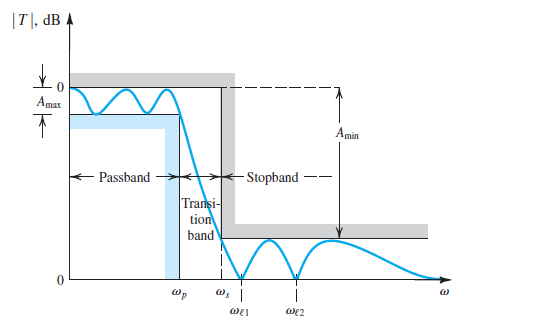
\includegraphics[scale=1]{figures/cProblemloesning/Lavpasfilter_generisk.PNG}
	\caption{På figuren ses et bodeplot filter, hvor de fire karakteristika $(min_{A})$, $(max_{A})$, $(\omega_p)$ og $(\omega_s)$ af et lavpasfilter er angivet. \cite{Carter2013}}
	\label{fig:Lavpasfilter_generisk}
\end{figure}
\noindent Med udgangspunkt i de enkelte parametre af lavpasfilteret kan den pågældende orden af filteret bestemmes vha. \eqref{eq:lavpasfilter} for overføringsfunktionen:
\begin{equation} \label{eq:lavpasfilter}
A(\omega_s) = 10 \text{log} \cdot \left[1 + \epsilon^2 \cdot (\frac{\omega _s}{\omega _p})^{2N}\right] 
\end{equation}

\noindent I \eqref{eq:lavpasfilter} betegner $A(\omega _s)$ den minimale dæmpning der kræves af stopbåndet. $(\omega_p)$ og $(\omega_s)$ er pasbåndfrekvensen og stopbåndfrekvensen, som begge er angivet i Hz. Disse variable kan ses på \figref{fig:Lavpasfilter_generisk}. N angiver filtrets orden, og $\epsilon$ er udtrykt ved nedenstående \eqref{eq:epsilon}:
\begin{equation}\label{eq:epsilon}
\epsilon = \sqrt{10^{A_{max} / 10} -1}
\end{equation}

Nu kan lavpasfilterets orden bestemmes, jævnfør værdierne fra kravspecifikationerne fra afsnit \ref{FilterAfs}, side \pageref{FilterAfs} ved at indsætte disse værdier i \eqref{eq:lavpasfilter}. Udregningerne vil se ud som følgende:
\begin{equation}
\epsilon = \sqrt{10^{3dB /10} -1} = 0.998 \\ \label{eq:orden}
14\text{dB} = 10 \cdot \text{log} \left[1 + \epsilon ^2 \cdot (\frac{45\text{Hz}}{25\text{Hz}})^{2N}\right] \\
N = 2.711 \approx 3
\end{equation}
\noindent Det fremgår af \eqref{eq:orden}, at lavpasfilterets orden bliver $3$. Filterets orden kun kan angives i hele tal og derfor afrundes resultatet. Hvis kravene til filteret skal overholdes, skal der altid rundes opad ved udregning af orden.

Der skal altså benyttes et 3. ordens lavpasfilter. I dette tilfælde anvendes filtertypen, SKT. Et 3. ordens lavpasfilter konstrueres ved at sammenætte et 1. ordens filter med et 2. ordens filter. Af figur \figref{fig:SallenKey1} og \figref{fig:SallenKey2} fremgår hhv. et 1. og 2. ordens lavpasfilter designet efter SKT. \cite{Carter2013}
	
\begin{figure}[H]
	\centering
	\begin{minipage}[b]{0.45\textwidth}
		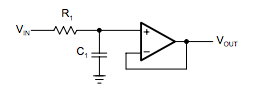
\includegraphics[width=\textwidth]{figures/cProblemloesning/Lavpasfilter1_teoretisk.PNG}
		\caption{På figuren ses en illustration af et 1. ordens unity-gain Sallen-Key lavpasfilter, hvor værdien C er kondensatoren, R er modstandene. filterKonfigurationen har en indgangsspænding, Vin og udgangsspænding, Vout. \citep{Carter2013}}
		\label{fig:SallenKey1}
	\end{minipage}
	\hfill
	\begin{minipage}[b]{0.45\textwidth}
		\includegraphics[width=\textwidth]{figures/cProblemloesning/Sallenlavpas.PNG}
		\caption{På figuren ses en illustration af et 2. ordens unity-gain Sallen-Key lavpasfilter, hvor værdien C er kondensatoren, R er modstandene. filterKonfigurationen har en indgangsspændings, Vin og en udgangsspænding, Vout. \citep{Carter2013}}
		\label{fig:SallenKey2}
	\end{minipage}
\end{figure}

I designet af et 3. ordens filter designes både et 1. og et 2. ordens filter i forlængelse af hinanden, som ses på \figref{fig:filter_Orden}.
\begin{figure}[H]
	\centering
	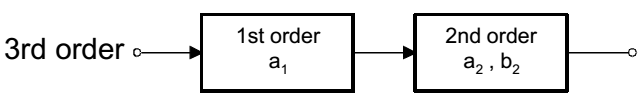
\includegraphics[scale=1]{figures/cProblemloesning/Filter_Orden.PNG}
	\caption{På figuren ses, hvordan et 3. ordens filter designes ved et 1.- og 2. ordens filter i forlængelse af hinanden. Værdierne $a_{1}$, $a_{2}$ og $b_{2}$ er fastsatte værdier, som kan aflæses i en tabel for Butterworth koefficienterne. \cite{Carter2013}}
	\label{fig:filter_Orden}
\end{figure}
\noindent Filtret designes efter SKT-metoden bestående af tre modstande, tre kondensatorer og to operationsforstærkere. Værdierne for modstandene kan udregnes ved \eqref{eq:Lavpas1Modstande} for et 1. orden lavpasfilter, der skal benytte en modstand, kondensator og operationsforstærker. I \eqref{eq:LavpasModstande} udregnes modstandene for et  2. orden lavpasfilter, der skal benytte to modstande, to kondensatorer og en operationsforstærker. \cite{Carter2013}
\begin{equation} \label{eq:Lavpas1Modstande}
R_{1} = \frac{a_1}{2 \cdot \pi \cdot f_c \cdot C_1} \\
\end{equation}
\begin{equation}
 \label{eq:LavpasModstande}
R_{2,3} = \frac{a_2 \cdot C_3 \pm \sqrt{{a_2}^2 \cdot C_3^2 - 4 \cdot b_2 \cdot C_2 \cdot C_3}}{4 \pi \cdot f_c \cdot C_2 \cdot C_3}
\end{equation}
\noindent Værdien for $C_{1}$ i \eqref{eq:Lavpas1Modstande} og \eqref{eq:LavpasModstande} er nødvendigvis ikke det samme, da disse to ligninger er uafhængige af hinanden. Der aflæses i en tabel for Butterworth koefficienterne, at $a_{1}$, $a_{2}$ og $b_{2}$ skal være 1.0000. For at finde reelle værdier under kvadratroden i \eqref{eq:LavpasModstande} skal følgende være opfyldt:
\begin{equation} \label{eq:kondensator}
C_3 \geq C_2 \frac{4 \cdot b_2}{a_2^2}
\end{equation}
I \eqref{eq:LavpasModstande} står C for kondensatorer, R står for modstande og $a_1$ og $b_1$ er konstanter, mens $f_c$ er den valgte knækfrekvens i Hz, jævnfør kravspecifikationerne afsnit \ref{FilterAfs} på side \pageref{FilterAfs}. 

\noindent For at udregne modstandene fastsættes $C_1$ til 100nF for hhv. både 1. og 2. ordens lavpasfiltrene. Når $C_1$ er bestemt, kan $C_2$ for 2. ordens lavpasfilteret beregnes ved at benytte følgende \eqref{eq:kondensator}. Som grundregel skal $C_3$ være over dobbelt så stor som $C_2$:
\begin{equation}  
C_3 \geq 100\text{nF} \frac{4\cdot 1}{1.000^2} = C_3 \geq 400\text{nF}
\end{equation}

\noindent Ud fra ovenstående ligning vælges $C_3$ til at være 470nF for at opfylde \eqref{eq:kondensator}. Når værdierne for C er bestemt kan modstandene for filteret bestemmes. For et 1. orden lavpasfilter benyttes \eqref{eq:Lavpas1Modstande} til at beregne $R_1$ og for et 2. ordens lavpasfilter anvendes \eqref{eq:2ordenmodstand} for at beregne $R_1$ og $R_2$. 
\begin{equation} \label{eq:1ordenmodstand}
R_{1} = \frac{1}{2 \cdot \pi \cdot 25 \cdot 100nF} R_{1} = 63661.98 \Omega
\end{equation}
\begin{equation} \label{eq:2ordenmodstand}
R_{2,3} = \frac{1.0000 \cdot 470\text{nF} \pm \sqrt{1.0000^2 \cdot 470\text{nF}^2 - 4 \cdot 1.0000 \cdot 100\text{nF} \cdot 470\text{nF}}}{4 \pi \cdot 25\text{Hz} \cdot 100\text{nF} \cdot 470\text{nF}} = \begin{cases} R_{2} = 19546.69414 \Omega \\ R_{3} =  44115.28306 \Omega \end{cases}
\end{equation}
\noindent Filterets værdier for kondensatoerne og modstandene er nu udregnet for hhv. 1. og 2. ordens filter. Filterkonfigurationen kan nu simuleres i LTspice for at bestemme, hvor godt et 3. ordens filter, der er blevet designet.

\begin{figure}[H]
	\centering
	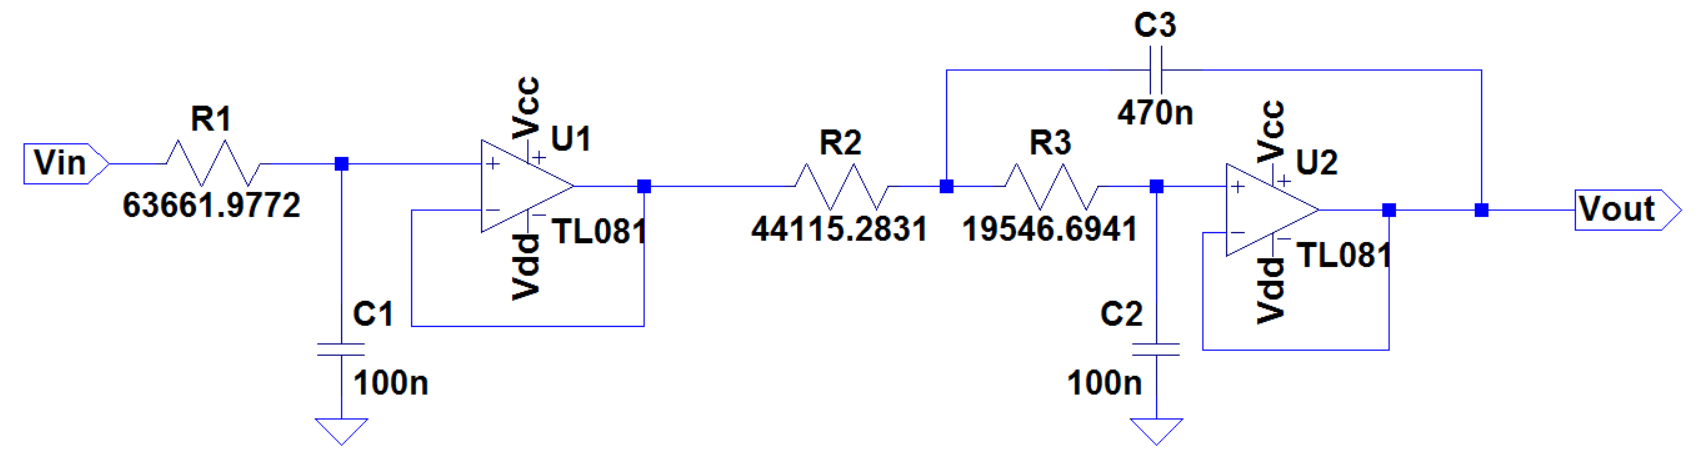
\includegraphics[scale=0.3]{figures/cProblemloesning/Lavpasfilter1_LTspice.PNG}
	\caption{På figuren ses det teoretiske kredsløb for lavpasfilteret med udregnede værdier for de enkelte modstande og kondenstatorer. Filteret er designet i LTspice.}
	\label{fig:lavpasfilter1_LTspice}
\end{figure}

\subsubsection{Simulering}
For at udføre en simulering af 3. ordens lavpasfilteret, foretages en AC-analyse, der beskriver forholdet mellem frekvensindholdet og filterets dæmpning. Kredsløbet simuleres med et inputsignal, der har en amplitude på $1$V. Der foretages en simulering ud fra kravspecifikationerne i afsnit \ref{FilterAfs} på side \pageref{FilterAfs}. LTspice anvendes til simulering af lavpasfilteret, hvor der anvendes operationsforstærkeren, TL081, hvilket er den operationsforstærker, der også vil blive benyttet i test af filteret. I simuleringen vil der blive undersøgt, hvorledes kravene stemmer overens med kravspicifikationerne, ved at betragte et bodeplot over det simulerede 3. ordens filter.

\begin{figure}[H]
	\centering
	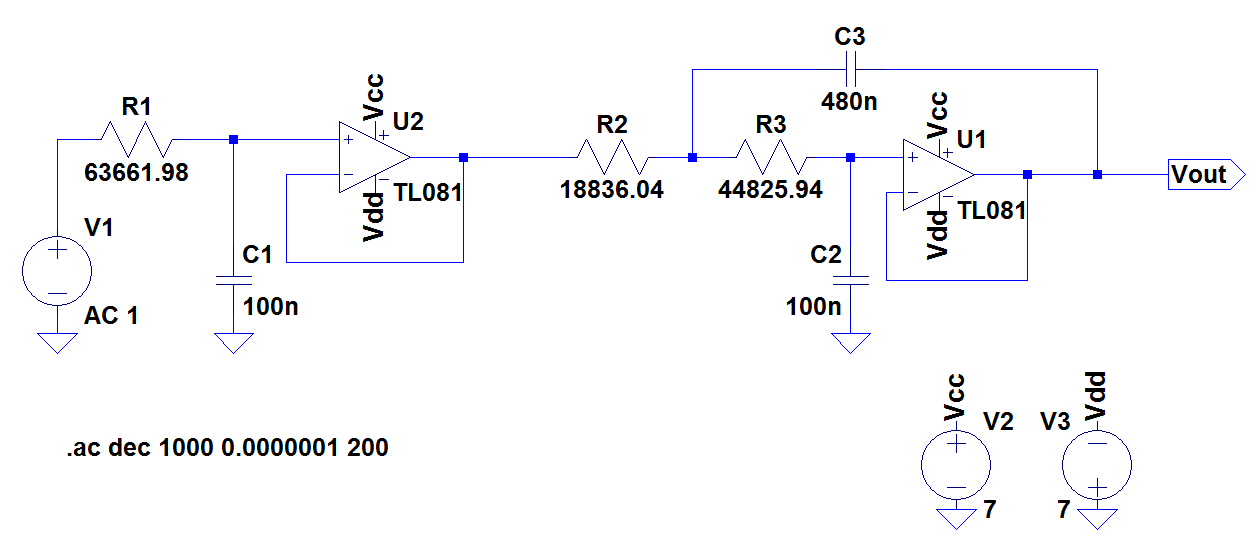
\includegraphics[scale=0.45]{figures/cProblemloesning/Lavpasfilter_LTspice.PNG}
	\caption{Af figuren fremgår en illustration af kredsløbet for et 3. ordens lavpasfilter. Filteret simuleres i LTspice vha. en AC-analyse med et inputsignal, der har en amplitude på $1$V.}
	\label{fig:lavpasfilter_LTspice}
\end{figure}

\begin{figure}[H]
	\centering
	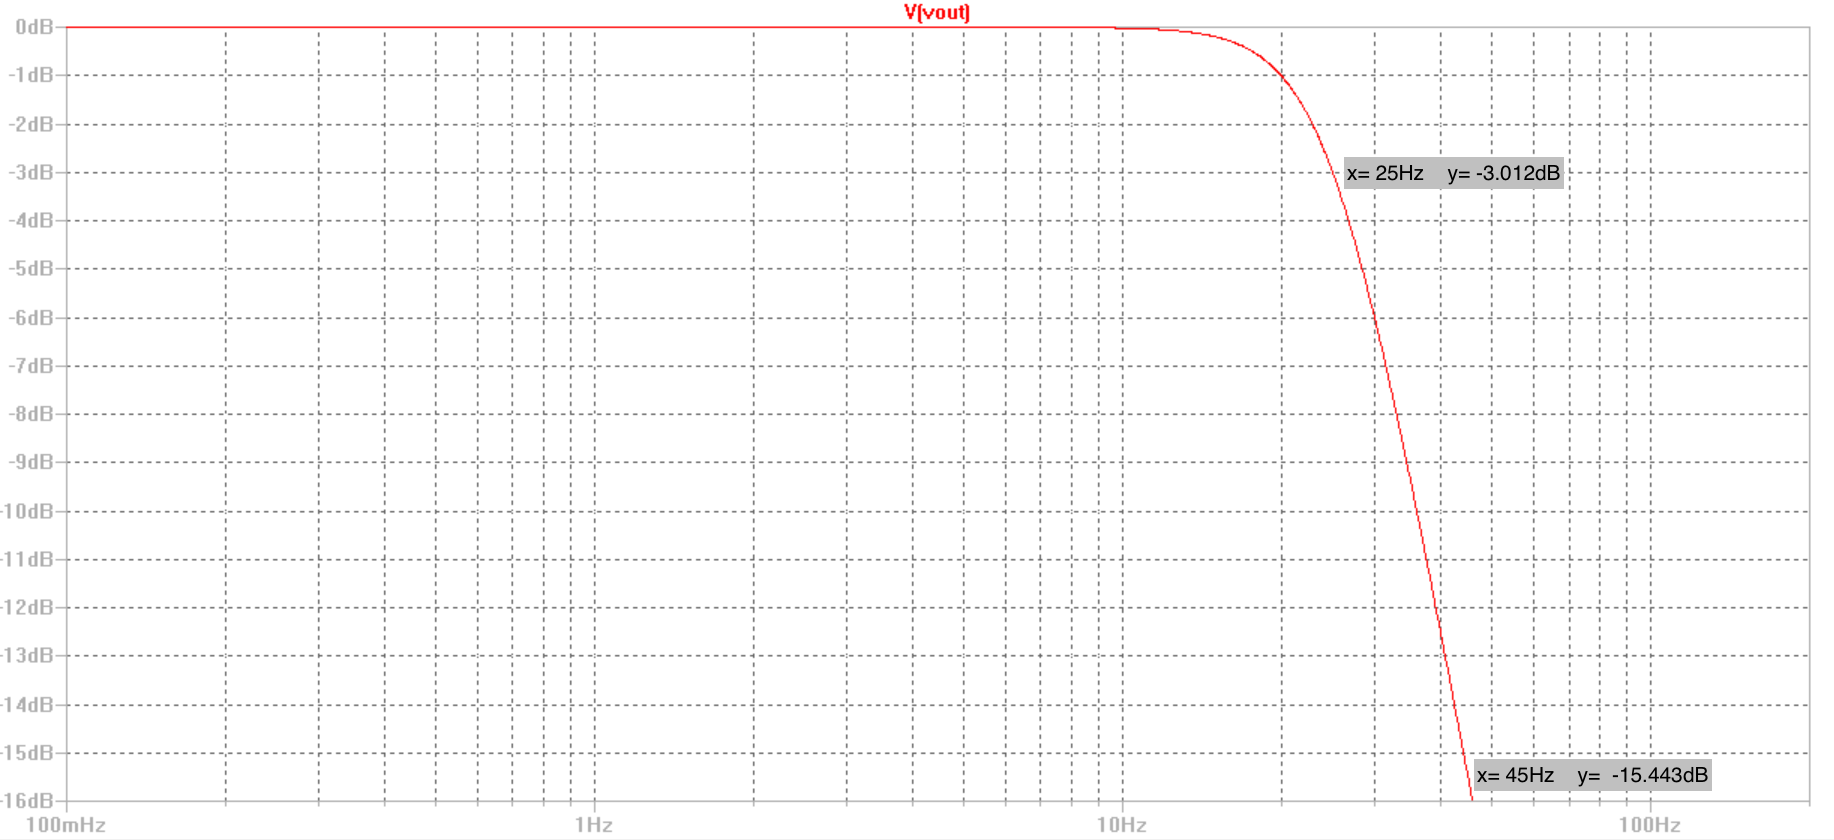
\includegraphics[scale=0.4]{figures/cProblemloesning/Lavpasfiltergraf_LTspice1.PNG}
	\caption{Af figuren fremgår en illustration på et bodeplot, der viser 3. ordens filterets frekvensindhold målt i Hz over dæmpningen målt i dB. Lavpasfilteret er simuleret i LTspice.}
	\label{fig:lavpasfilter_LTspice}
\end{figure}
\noindent Af bodeplottet fremgår det, at det simulerede filter har en maksimal amplitude i db på $-3.012$ ved en knækfrekvens på $25$Hz, hvilket ikke overholder kravspecifikationerne i afsnit \ref{FilterAfs}, side \pageref{FilterAfs}. Grundet den lave afvigelse accepteres afvigelsen i midlertidigt og der udføres derfor endnu en simulering af filteret med de reelle modstande, der kan benyttes under implementeringen. Der aflæses, at der ved en stopbåndsfrekvens på $45$Hz er amplituden i db på $-15.443$. Dette overholder projektets opstillede krav for filterkonfigurationen ved en minimum dæmpning på $14$ dB i stopbåndsfrekvensen. Filterkonfigurationen med reelle modstande fremgår af nedenstående \figref{Sim_reel_modstande}. Reelt findes de udregnede modstande ikke, hvorfor der benyttes de modstande der kommer tættest på den teoretiske værdi. 

%\begin{figure}[H]
%	\centering
%	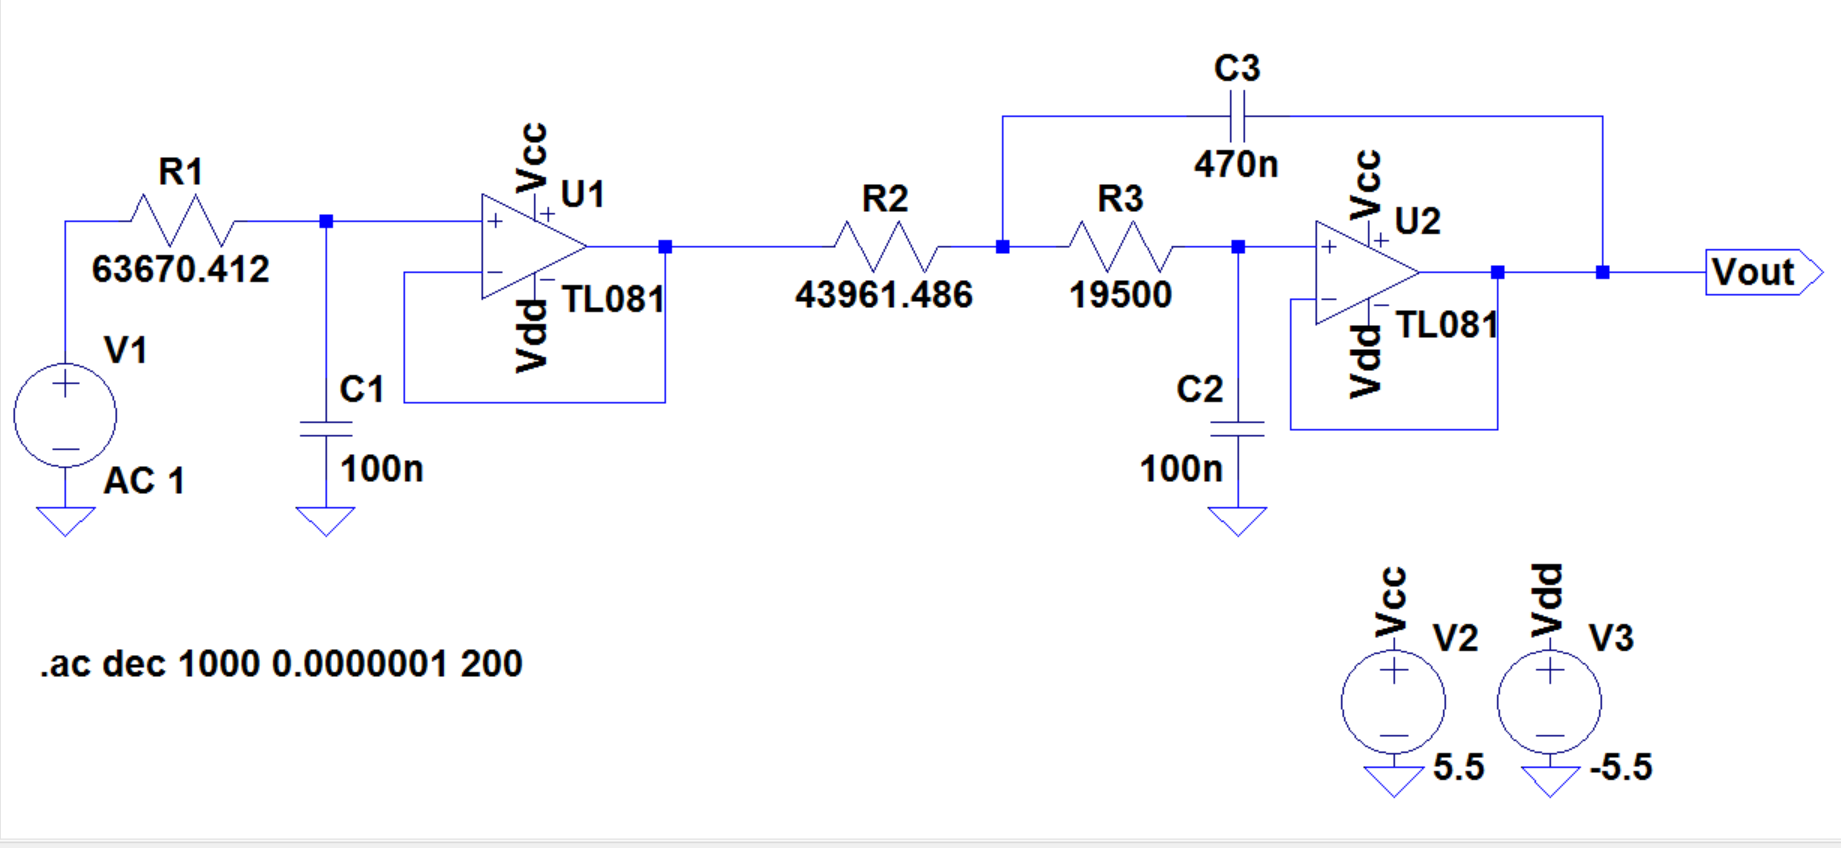
\includegraphics[scale=0.4]{figures/cProblemloesning/Sim_reel_modstande.PNG}
%	\caption{Af figuren fremgår et 3. ordens filter med reelle modstande, hvor R$1$ er parallel med $68$K $\Omega$ og $1$M $\Omega$, R$2$ er er parallel med $47$K $\Omega$ og $680$K $\Omega$ og R$3$ er parallel med to $32$K $\Omega$ modstande.}
%	\label{fig:Sim_reel_modstande}
%\end{figure}
%
%\begin{figure}[H]
%	\centering
%	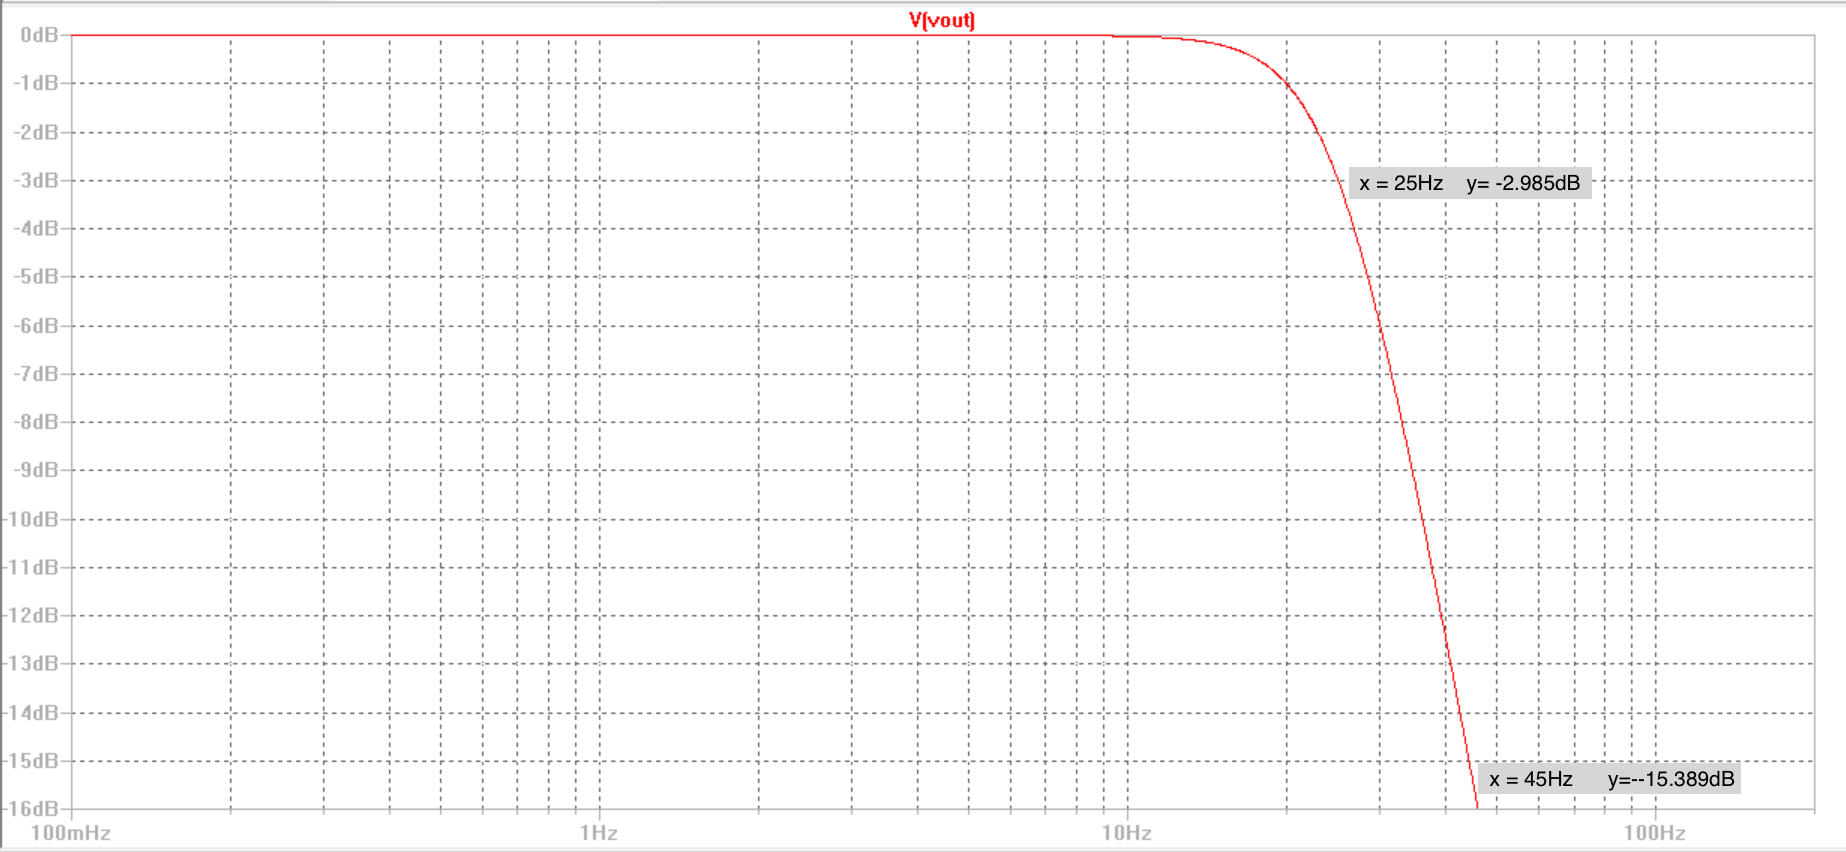
\includegraphics[scale=0.4]{figures/cProblemloesning/Sim_reel_graf.PNG}
%	\caption{Af figuren fremgår en illustration af et bodeplot, der viser 3. ordens filterets frekvensindhold målt i Hz over dæmpningen målt i dB med reelle modstande. Lavpasfilteret er simuleret i LTspice.}
%	\label{fig:Sim_reel_graf}
%\end{figure}

\noindent af bodeplottet det, at det simulerede filter med reelle værdier har en maksimal amplitude i dB $-2.985$ ved en knækfrekvens på $25$Hz, hvilket overholder kravspecifikationerne i afsnit \ref{FilterAfs}, side \pageref{FilterAfs}. Der aflæses, at ved stopbåndsfrekvensen på $45$Hz er amplituden i db $-15.389$, hvilket fortsat er acceptabelt ift. kravspecifikationerne for filterkonfigurationen. 

\subsubsection{Implementering og test} 
Der ses på \figref{fig:lavpasfilter_LTspice} at der benyttes 3 modstande og 2 kondensatorer til at designe kredsløbet. Af \tableref{Tab:Maalingfilter} fremgår, hvorledes modstandene sammensættes for at få de ønskede værdier, der fremgår i \figref{Sim_reel_modstande}, samt modstandenes afvigelse fra de ideelle modstande. For at finde afvigelsen er der foretaget målinger på tre ens reelle modstande og kondensatorer og på denne måde vurderes det, hvilke komponenter, der afviger mindst fra de teoretiske værdier. Dette er ydermere illustreret i \tableref{Tab:Maalingfilter}.
\begin{table}[H]
	\centering
	\begin{tabular}{|l|l|l|l|}
		\hline
		\textit{}                                     & \textit{Teoretisk} & \textit{Måling}    & \textit{Afvigelse} \\ \hline
		\multirow{2}{*}{\textit{$R_{1}$(Parallel) :}} & $1$M$\Omega$       & $1.0046$M$\Omega$  & $0.46\%$           \\ \cline{2-4} 
		                                              & $68$K$\Omega$      & $68.0350$K$\Omega$ & $0.05\%$           \\ \hline
		\multirow{2}{*}{\textit{$R_{2}$(Parallel) :}} & $680$K$\Omega$     & $1.0037$K$\Omega$  & $0.37\%$           \\ \cline{2-4} 
	                                               	  & $47$K$\Omega$      & $47.0540$K$\Omega$ & $0.11\%$           \\ \hline
		\multirow{2}{*}{\textit{$R_{3}$(Parallel) :}} & $32$K$\Omega$      & $17.9600\Omega$    & $0.22\%$           \\ \cline{2-4} 
		                                              & $32$K $\Omega$     & $816\Omega$        & $0.49\%$           \\ \hline
		\textit{$C_{1}$ :}                            & $100$n             & $98$n              & $2.00\%$           \\ \hline
		\textit{$C_{2}$ :}                            & $470$n             & $464$n             & $1.29\%$           \\ \cline{2-4} 
		\textit{$C_{3}$ :}                            & $100$n             & $98$n              & $2.00\%$           \\ \hline
	\end{tabular}
	\caption{I tabellen ses der, at de anvendte modstande og kondensatorer afviger fra den teoretiske værdi, hvilket er forventet af reelle komponenter. Det er en acceptabel afvigelse, så modstandene kan derfor anvendes til implementering}
	\label{Tab:Maalingfilter}
\end{table}
Herefter implementeres kredsløbet. I testen anvendes en spændingsforsyning på $5.5$V og en funktionsgenerator som inputsignal, samt et multimeter til aflæsning af dæmpningen. Funktionsgeneratoren sættes til de ønskede frekvenser i intervaller af $1$Hz fra $10$Hz til $50$Hz. Outputtet i dB måles for hver frekvens. Ud fra disse målinger plottes en graf af dæmpningen i MatLab, hvilket er illustreret på \figref{fig:Lavpas_Matlab}.  

\begin{figure}[H]
	\centering
	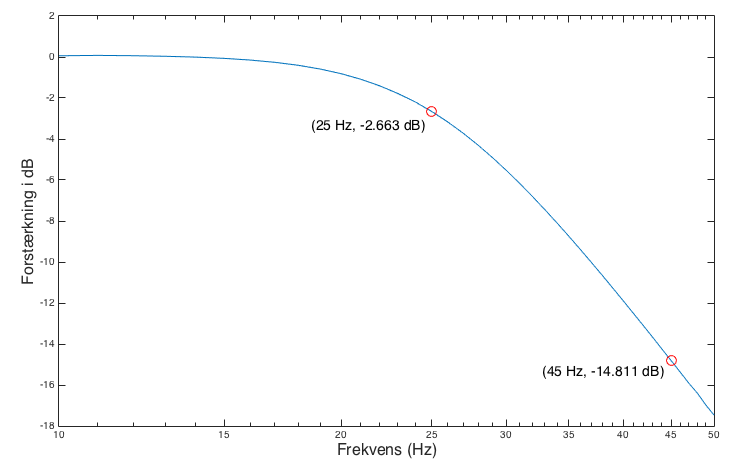
\includegraphics[scale=0.4]{figures/cProblemloesning/Lavpas_Matlab.PNG}
	\caption{Figuren viser dæmpningen som en graf over de målte frekvenser i Hz som funktion af outputtet i dB. På grafen er der angivet knækfrekvens og stopbåndfrekvens}
	\label{fig:Lavpas_Matlab}
\end{figure}

\noindent Sammenlignes værdierne fra \ref{fig:Lavpas_Matlab} for det testede kredsløb med værdierne fra \ref{fig:lavpasfilter_LTspice} for det simulerede kredsløb ses der en ændring i frekvens og dæmpning, hvilket også er forventet grundet andre kodensatorer og modstande. 

\begin{table}[H]
	\centering
	\begin{tabular}{|l|l|l|l|}
		\hline
  & \textit{Simulering} 	& \textit{Test}  &\textit{Afvigelse} \\ \hline
Knækfrekvens	 & $25Hz$ 			& $25.0308Hz$			& $4\%$  \\ %\hline
Stopbåndsfrekvens & $45Hz$		& $45.0816Hz$			& $0.18\%$ \\ \hline
Dæmpning på stopbånd & $15.489dB$  & $14.881dB$     & $9.61\%$  \\ \hline
Dæmpning på pasbånd & $3.0273dB$	  & $2.663dB$  & $13.68\%$  \\ \hline
	\end{tabular}
	\caption{I tabellen ses afvigelserne for hhv. knækfrekvens, stopbåndsfrekvens og dæmpning af stopbånd og pasbånd ift. simlering og test}
	\label{Tab:Afvigelse_simulering}
\end{table}

\noindent Ud fra de testede værdier i \tableref{Tab:Tolerance} og kravspecifikationer i afsnit \ref{FilterAfs} på side \pageref{FilterAfs} er der er ingen afvigelse på knækfrekvensen og stopbåndsfrekvensen. Der er en variation ift. dæmpningen for både stop- og pasbånd på hhv. $6.36\%$ og $8.37$\% i forhold til kravet.

\begin{table}[H]
	\centering
	\begin{tabular}{|l|l|l|l|}
		\hline
   & \textit{Krav} 	& \textit{Test}  &\textit{Afvigelse} \\ \hline
Knækfrekvens	 & $25Hz$ 			& $25Hz$			& $0\%$  \\ \hline
Stopbåndsfrekvens & $45Hz$		& $45Hz$			& $0\%$ \\ \hline
Dæmpning på stopbånd & $14dB$    & $14.8910dB$    & $6.36\%$  \\ \hline
Dæmpning på pasbånd & $3dB$		& $2.7490dB$	    & $8.37\%$ \\ \hline
	\end{tabular}
	\caption{I tabellen ses afvigelserne for hhv. knækfrekvens, stopbåndsfrekvens og dæmpning af stopbånd og pasbånd ift. krav og test}
	\label{Tab:Tolerance}
\end{table}
\noindent I forhold til tolerancekravene i afsnit \ref{FilterAfs} på side \pageref{FilterAfs} skulle dæmpningen på stopbåndet være minimum $14 dB$ og måtte maksimalt have en afvigelse herfra på $+10\%$. Denne tolerance overholdes ved testen, da de acceptable dæmpningsværdier vil ligge i intervallet $14$-$15.4$db. For pasbåndet skulle dæmpningen maksimalt være $3$dB med en maksimal afvigelse på $-15\%$. Dette vil sige at testen passer inden for tolerancekravene, da der accepteres værdier i intervallet $2.55$-$3$dB. På baggrund af dette accepteres alle målte afvigelser ved testen af filteret.